\chapter{Lecture 1: Why Study Robot Dynamics?}\label{lecture1}
\section{Background / Motivation}
The \textbf{motivation} for this course is to
\begin{itemize}
\item Build great robots that can do amazing things
\item Exploit natural dynamics of robots, not just doing dump control
\item Achieve extraordinary performance in terms of speed, efficiency, or robustness (Honda's ASIMO vs. passive dynamic walkers)
\item Controlling nonlinear systems without complete control authority
\item View computation of challenging tasks in robotics (manipulation, autonomous driving) through the lense of dynamics.
\end{itemize}
This course is all about nonlinear dynamics and control of underactuated mechanical systems, with an emphasis on computational methods. Especially it covers the \textbf{topics}
\begin{itemize}
\item Nonlinear dynamics
\item Applied optimal and robust control
\item Motion planning
\item Examples from biology and applications to legged locomotion, compliant manipulation, underwater robots, and flying machines
\end{itemize}

\section{Definitions}
Nonlinear differential equations typically take the form
$$ \dot{x} = f(x,u) $$
where $f$ is a vector valued function, $x$ is the state vector and $u$ is the vector of control input and $\dot{x}=\frac{dx}{dt}$ is the time derivative.
Mechanical Systems are described by second order differential equations. When the state vector is defined as 
$$x=\begin{bmatrix}q \\ \dot{q}\end{bmatrix},$$ 
where the system dynamics can be described as
$$\ddot{q}=f(q,\dot{q}, u).$$
Since mechanical systems are \textit{control affine}, this specializes to
$$ \ddot{q}=f_{1}(q,\dot{q})+f_{2}(q,\dot{q})u.$$
A system of this form is called \textit{underactuated} if $rank[f_{2}]<=n$. 
Other causes of underactuated include
\begin{itemize}
\item Input saturation (e.g. torque limits)
\item State constraints (e.g. joint limits)
\item Model uncertainty / state estimation
\end{itemize}
 
\section{Manipulator Equations}
The equations of motion for simple systems, e.g. a double pendulum, are quite simple to derive. Results, e.g. obtained from an Lagrangian calculation approach, can be expressed in the form of the standard "manipulator equations":
$$M(q)\ddot{q}+C(q,\dot{q})\ddot{q}=\tau_{g}(q)+Bu$$ 
where $M$ is the Inertia matrix, $C$ is the matrix of Coriolis terms $\tau_{g}$ covers gravitational torques, $B$ maps inputs to generalized force and u is the control input (either force or torque).

The acceleration then is expressed as
\begin{equation}\label{eq:eom_dbl_pendl}
\ddot{q}=M^{-1}(q)[\tau_{g}(q)+Bu-C(q,\dot{q})\dot{q}].
\end{equation}
With equation \ref{eq:eom_dbl_pendl}, the dynamics of the systems and accordingly the functions $f_{1}$ and $f_{2}$ are fully defined.

For simulating the dynamics of a robot, it is sufficient to provide the  kinematics in form of a \textit{URDF file}, pass it to an forward Dynamics solver and you get the resulting acceleration and its integrations.

\section{Plan for the Course}

\begin{figure}[h!]
\begin{center}
  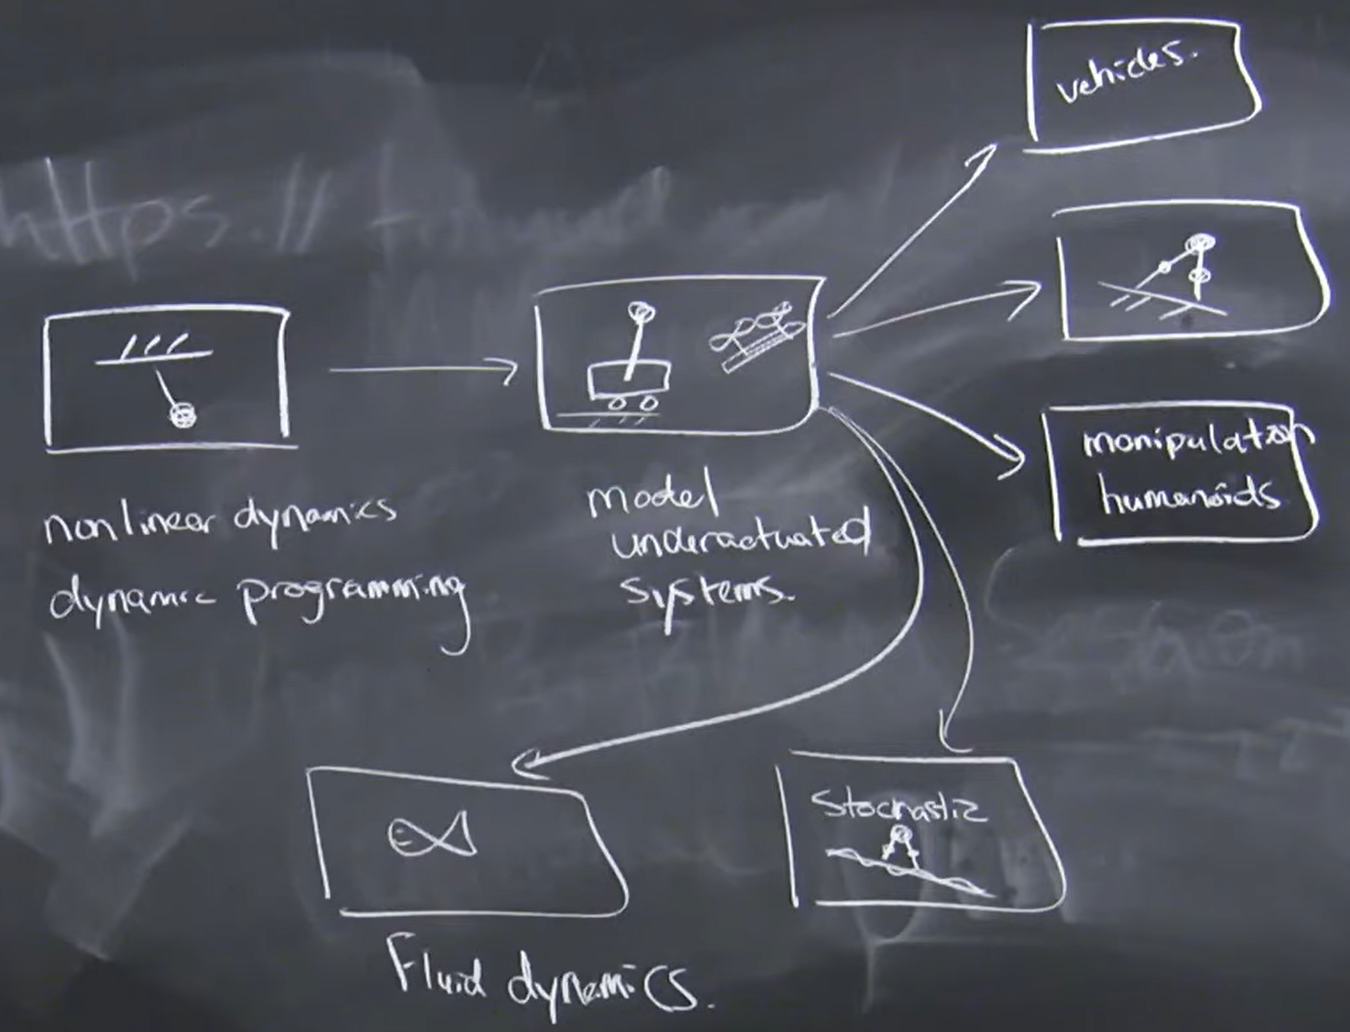
\includegraphics[width=1\textwidth]{Figures/courseOverview.png}
  \caption{Course overview: Basics first, then simple systems and then various advanced systems.}
  \label{fig:overview}
\end{center}
\end{figure}